In this chapter, we present the background and motivation of our thesis.
We start with our background in medical procedures, looking at how doctors perform colonoscopies, mainly from a gastrointestinal perspective.
After this, we then look at what the objective is for the medical staff, with different anomalies in the GI tract. Then, we shift our focus to how doctors use computer-aided diagnosis (CAD) today to help with the screening. 

After the discussion from a medical point of view, we shift our focus to machine learning and give a brief introduction to different machine learning methods. We look at how machines can ``learn'' and discuss different areas we can use and the areas we are using machine learning today. We then go in depth into the examples and look at the most common machine learning models. We look at the most state of the art form of machine learning, namely neural networks, and look into the most frequent use case of this type of algorithm.
With this in mind, we look at neural networks, especially convolutional neural networks, and how they work.
Lastly, we combine the need for computer-aided diagnosis with machine learning, looking at where previous models fall short and why that is the case.

\section{The Medical Background}
As we recall from the introduction, our motivation for this thesis is the improvement of medical diagnosis, more specific CAD. 
Before we look into the CAD procedures that are in use today, we need to go more in-depth into the capture of the medical images. 


\subsection{Endoscopy and Colonoscopy}
\label{cha:endocolo}
Gastrointestinal endoscopies are one of the most routine medical examinations where medical staff visualise the mucosa of the patient via a camera through the GI tract~\cite{Holme13}.
Today the medical staff working with the visual screening of the intestinal tract use primarily two different methods: colonoscopy and gastroscopy. 
Colonoscopy is the practice of inserting a colonoscope into the rectum and moving through the large intestine towards the small intestine.  Gastroscopy is the practice of inserting a camera via the mouth to get a visualisation through the stomach.

The endoscopic tool used for this visualisation is made out of a flexible tube with a charged coupled device (CCD) working as a camera at the end. In addition to the light sensing chip, there is also an optical fibre to transport light to the camera. At the other end, the colonoscope is connected to a device that records the video, and a light source for the optical fibre. The video from the CCD is shown live for the medical staff for the doctors to analyse~\cite{Colonoscope}.
As Figure \ref{fig:HumanGI}\footnote{From \url{https://commons.wikimedia.org/wiki/File:Stomach_colon_rectum_diagram-en.svg}.} shows, the colonoscope can either be inserted into the anus, and traverse up the colon, or it can be inserted through the stomach, and traverse through the small intestine.


\begin{figure}[h]
	\centering
	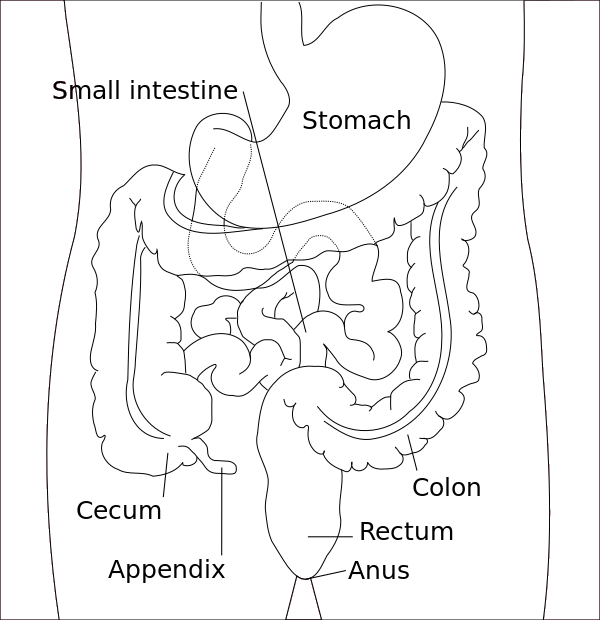
\includegraphics[scale=0.4]{background/figures/Stomach_colon_rectum_diagram.png}
	\caption{Diagram of the human GI tract}
	\label{fig:HumanGI} 
\end{figure}



\subsection{Summary}
We have now looked at the medical perspective of colonoscopy. We see that the practice has not changed since the introduction of the colonoscope and that the best chance of detection is manually looking at images by professional medical staff. \todo{Need more here, or in previous section.. Remember to talk about medical team}


\section{CAD - Computer Aided Diagnosis}
\label{cha:CAD}
In the previous section, we gave a summary of the medical procedure associated with a colonoscopy. We described the tool used for colonoscopy,  and the need for a medical team to support during the procedure.
The research into better systems for automation and detection has been prevalent in the twenty-first century.  This shift towards CAD is an essential move, given the invasiveness and stress associated with medical colonoscopies, and the more confident we are in the findings of anomalies during the procedure, the higher chance of a patient not getting cancer due to the missed anomalies.
Despite the effort by the medical staff, on average, 20\% of polyps are either missed or incompletely removed~\cite{kaminski2010quality}. Given the increase in cancer risk, this is highly undesirable.
In addition to the possible miss chance during colonoscopies, the price of the procedures is high despite its importance. In the US a colonoscopy can cost 1000 dollars, and the annual cost for every examination is more than 10 billion dollars~\cite{NYT_cancer, NYT_cancer2}.

The motivation for this thesis is to advance the systems in place that does CAD, and in more detail, we want to improve the medical systems for detecting polyps in the GI tract. 
Automatic detection of polyps is, in general, a well-researched study, and at the time there are many publications regarding this detection and classification, especially when it comes to generalisation and limited datasets~\cite{riegler2016multimedia}.  
Despite the numerous papers published on the subject, there are still challenges that need more research. 
\vspace{5px}
Wang et al. published a system called Polyp-Alert that provides near real-time feedback during colonoscopy~\cite{wang2015polyp}. The system correctly detected 97\% (42 of 43) of the polyps in the videoes provided. The system had a 4.3\% error, marking non-polyps as polyps. Polyp-Alert shows that we already have fast, effective and potentially useful colonoscopy tools to guide medical staff.

When it comes to network training,  Tajbakhsh et al. demonstrated how fine-tuning a pretraind convolutional neural network in a layer-wise manner leads to incremental performance improvement in medical images~\cite{DBLP:journals/corr/TajbakhshSGHKGL17}.

In 2016 Pogorelov et al. presented a complete end-to-end multimedia system for tackling automatic analysis of GI tract videos. The proposed system includes a pipeline ranging from data collecting, processing and data analysis, to visualisation~\cite{Pogorelov2017}. 

Pogorelov et al. also recently published a paper on the generalisation of data, for the purpose of using open datasets for training CAD systems~\cite{pogorelov2018deep}. In this paper, they presented hand-crafted and deep learning-based methods for detection of polyps in videos from colonoscopies. In this paper they worked to achieve real-world comparability by using challenging datasets captured with different kinds of hardware. In addition to this, they used imbalanced datasets and as little as possible training data.
Their best model, a Generative adversarial network for handcrafted features, reached a detection specificity of 94\% and an accuracy of 90.9\%, done with only 356 training samples.

As mentioned in the introduction, Hicks et al. published the Mirmir system~\cite{25953}. 
Mirmir has, since the creation been analysed and, in later papers, shown that the system has similar problems to the one that we encounter~\cite{25956}.  
\todo{´´Future works'' in Stevens paper is the basis for this thesis}
\todo{Steven: I want to discuss this with you.}



    
\section{Machine Learning}
We have looked at the challenges that the medical staff has when it comes to detecting polyps, and how it is solved today.
However, to truly understand how automated systems like Mirmir~\cite{25953} works, we need to look at how machine learning helps with the detection of the anomalies the medical staff are searching for.  

Machine learning is a broad term, but we summarise it with the quote from  Tom M. Mitchell in his machine learning book from 1997~\cite{MitchellTomM1997Ml}:\\
\vspace{10px}

\begin{quote}
 A computer program is said to learn from experience E with respect to some class of tasks T and performance measure P, if its performance at tasks in T, as measured by P, improves with the experience E.

\end{quote} 
\label{ML}


\vspace{10px}
A few things of note from this quote is the variables mentioned. Experience (E) is the stored knowledge the program has gotten. It is in most cases just numbers used to approximate a solution given input, to try to get it as close to the right answer. This approximation is made for every task (T) until we are happy with the result.
Lastly, to tell how well our program performs we need a measure (P) that tells us how far away from the desired output we got.
   
From this, we see that the goal of machine learning is to improve some performance P with experience. This behaviour is a mimicry of how humans learn, where we as humans in the real world need to practice on a task to improve it.
As the amount of experience increase, both for us and the machine, the performance of the task becomes better and better. We have seen that machine learning algorithms have become superior at solving some human tasks~\cite{silver2016mastering,OpenAI_dota,DBLP:journals/corr/HeZRS15}, given enough time and computing power. 
Projects like AlphaGO and OpenAI Five show that, given the right amount and type of data, our machine learning algorithms can solve the same problems humans solve.

Until now, we have talked about machine learning in broad terms at this point. We have drawn a parallel between how humans learn, and how machines gather experience.  Now, we will look into the most popular machine learning techniques, and show how the machine learning algorithms store the experience gathered.
 
\subsection{Machine learning types}
With a basis in the quote from the machine learning book from Tom Mitchell~\cite{MitchellTomM1997Ml}, we have a broad definition of what machine learning can be.
As long as we have a model trying to complete a task based on previous experience, it can be called machine learning. Though just like for humans, machine learning has multiple ways to gather and retain information.
Figure \ref{fig:ML_types} shows a chart over the three most common categories within the field of machine learning. 

    \begin{figure}[h]
        \centering
        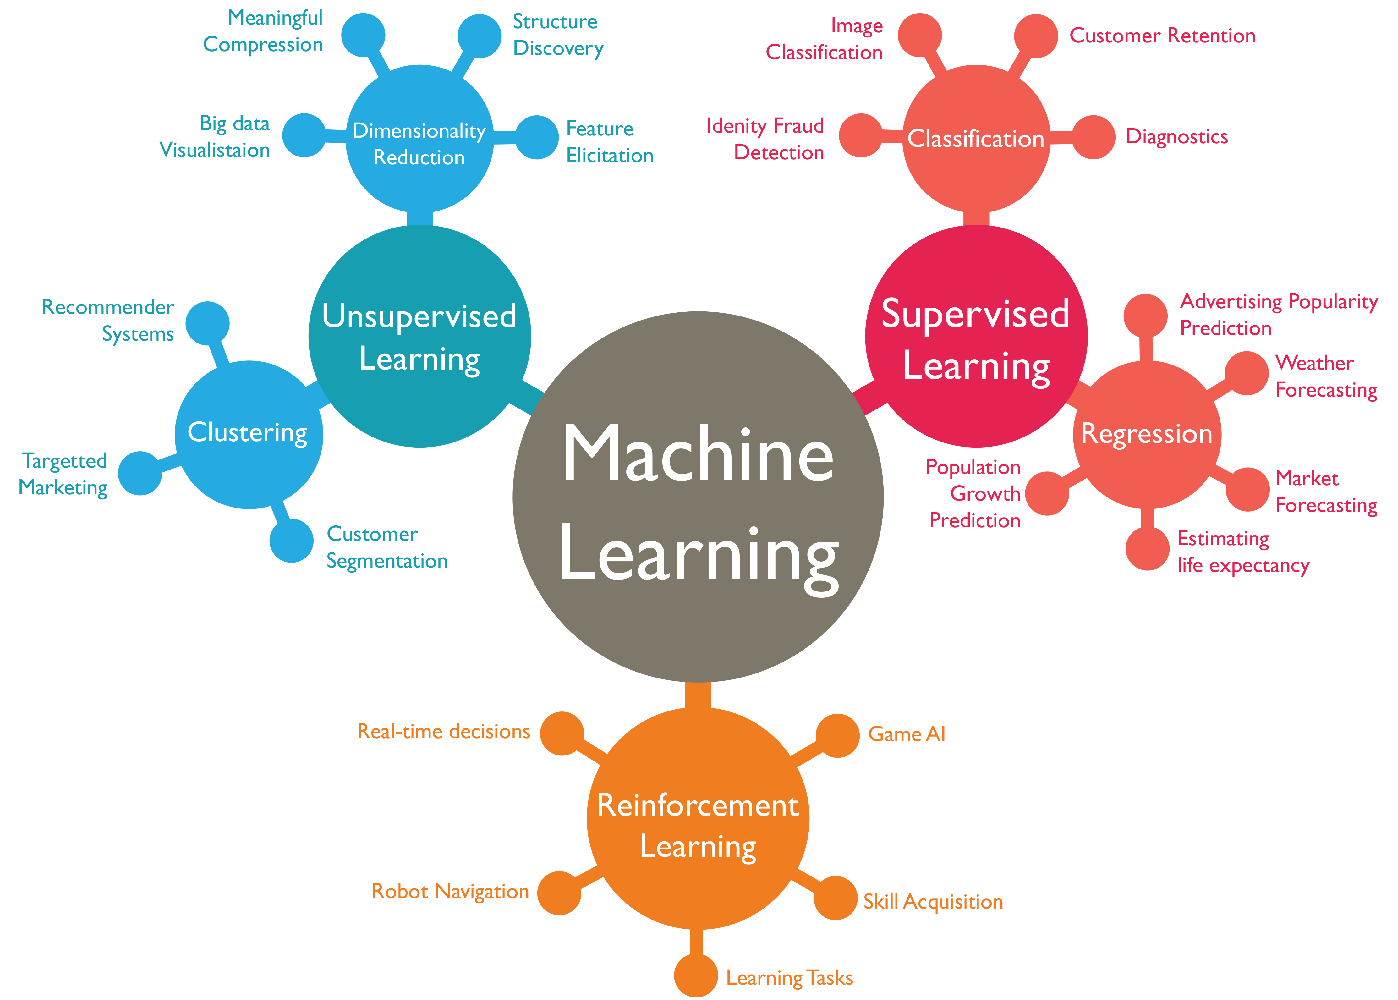
\includegraphics[width=\textwidth]{background/figures/ML_types.png}
        \caption{The three main types of machine learning and their most common subtypes}
    \label{fig:ML_types} 
    \end{figure}

We have three subcategories of machine learning: Supervised, Unsupervised, and Reinforcement learning. 
We will now present the three methods briefly. Then we will look at famous examples that helped shape machine learning types and algorithms we are using today.

\subsubsection{Supervised machine learning}
Supervised machine learning concerns the iterative process of labelling data based on previously labelled data.  Supervised machine learning functions have the objective of, given an input-output pair, approximate the input to be as close to the output.~\cite{AI:ModernApproach} Alternatively, in simplistic terms, given an input x, produce an answer as close as possible to the output y.
A supervised algorithm analyses the training data and produces an inferred function, which can be used to map new data entries. The two most common types of Supervised learning is shown in Figure \ref{fig:supervised_learning}.


Examples of supervised tasks are to recognise handwritten numbers, or differentiate between different car models. We consider a task supervised if the images come with the correct label in the data set. 
A more straightforward classification assignment is binary classification, where the target is (often, but not always) yes or no. Examples for binary classification is if an email is spam or not, is a car Norwegian or International.\todo{Her må det vere et storre skille mellom trening og evaluering. Tenk paa om det er smart aa omskrive dette} In the last example, the classification changes from binary to multi-class if we sort the cars on every nationality, and not just Norwegian/non-Norwegian. Another type concerning supervised learning tasks is regression. Regression is the act of prediction given prior data. Examples of regression are the prediction of stock prices, to estimating house prices or to predicting the weather.

An intuitive way to differentiate between the two supervised methods is to look at the output. If the output is a category or class from a predefined set, it is usually classification. If the output is an unbounded number, it is most likely regression. 
%\begin{figure}
%    \centering
%    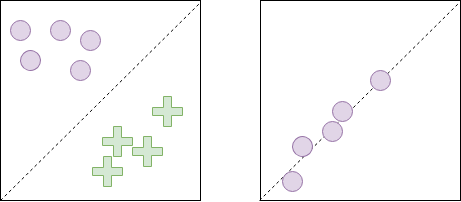
\includegraphics[scale=0.5]{figures/class_vs_reg.png}
%    \caption{The two main areas of supervised learning. \\ Left: Example of binary classification. Right: Example of regression} 
%\end{figure}
  
\begin{figure}
     \centering
     \begin{subfigure}[t]{0.34\textwidth}
         \centering
         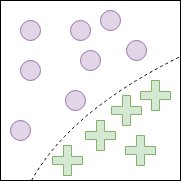
\includegraphics[width=\textwidth]{background/figures/supervised_classification.png}
         \caption{Supervised classification}
         \label{fig:supervised_calssification}
     \end{subfigure}
     \hspace{15px}
     \begin{subfigure}[t]{0.34\textwidth}
         \centering
         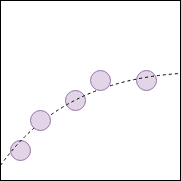
\includegraphics[width=\textwidth]{background/figures/supervised_regression.png}
         \caption{Supervised regression}
         \label{fig:supervised_regression}
     \end{subfigure}
        \caption{Examples of the two most common use cases for supervised learning}
        \label{fig:supervised_learning}
\end{figure}
\todo{Figures}
\FloatBarrier
\subsubsection{Unsupervised machine learning}
Unsupervised learning is the act of training without any supervision, in the sense that we do not give the algorithm the next output to the given input as we do in supervised learning. Figure \ref{fig:unsupervised_learning} shows a simplified concept of unsupervised learning.
Since we do not have categorised data in unsupervised learning, we often want the algorithms to find some underlying structure of the data, rather than classifying it.
Types of unsupervised learning can, for instance, be clustering or dimensionality reduction. In this context we define clustering as the act of sorting data based on similarity, and dimensionality reduction as the act of simplifying or compress the data.

An example of this can be if we want to sort plants based on similarity, or we are detecting anomalies in a dataset. We often use unsupervised learning for principal component analysis (PCA)~\cite{doi:10.1080/14786440109462720} or other dimensionality reduction methods.
A third method used in unsupervised learning is the adversarial route, where we use machine learning to make similar looking data to the original data set. 

 \begin{figure}[h]
     \centering
     \begin{subfigure}[t]{0.337\textwidth}
         \centering
         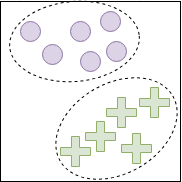
\includegraphics[width=\textwidth]{background/figures/unsupervised_clustering.png}
         \caption{Unsupervised clustering}
         \label{fig:unsupervised_clustering}
     \end{subfigure}
     \hspace{15px}
     \begin{subfigure}[t]{0.34\textwidth}
         \centering
         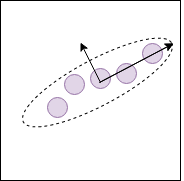
\includegraphics[width=\textwidth]{background/figures/unsupervised_PCA.png}
         \caption{Unsupervised dimensionality reduction}
         \label{fig:unsupervised_PCA}
     \end{subfigure}
        \caption{Examples of the two most common use cases for unsupervised learning}
        \label{fig:unsupervised_learning}
\end{figure}
      

\FloatBarrier
\subsubsection{Reinforcement Learning}
Reinforcement learning is the area in machine learning that is concerned with how a software agent should take actions.
The agent bases its actions on the environment, and it is influenced by the objective to get the maximum reward, as illustrated in Figure \ref{fig:reinforcement_learning}.
It is closely influenced by behaviourism, with the fact that the software agent wants to maximise the reward obtained continually. 

Successful types of reinforcement learning alogrithms are, for instance, Deep Recurrent Q-Learning~\cite{DBLP:journals/corr/HausknechtS15} or State–action–reward–state–action (SARSA)~\cite{Rummery94on-lineq-learning}.
\FloatBarrier

\begin{figure}[h]
        \centering
        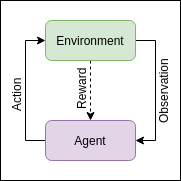
\includegraphics[width=0.34\textwidth]{background/figures/reinforcement.png}
        \caption{The basic structure of reinforcement learning}
        \label{fig:reinforcement_learning}
\end{figure}

%Reinforcement learning algorithms like these cannot be categorised under either supervised or unsupervised machine learning. \todo{more?}

\FloatBarrier
\subsubsection{Well known machine learning algorithms}
Now that we have a basis on the three types of machine learning we can go into more detail on the most successful types of machine learning used both now and in the past. 
Machine learning was coined as a term as early as in the 1950s by Alan Turing. The first concept was related to the Turing machine and is now considered a foreshadowing of genetic algorithms.~\cite{10.1093/mind/LIX.236.433}

\vspace{5px}

Forward to 1967, the Nearest Neighbour algorithm~\cite{Cover:2006:NNP:2263261.2267456} was created, which is considered the start of basic pattern recognition. The Nearest neighbour algorithm is a type of machine learning that requires no prior training, making it fast and deterministic.

\vspace{5px}

Another early adoption of machine learning was in the form of regression. Regression is the statistical concept of estimating the relationships among variables. It is in heavy use today, and one of the core concept we use machine learning.
Legendre first used regression in 1805 with his method of least squares\todo{MICHAEL OR PAAL:\\ How do I cite this? Should i find a ´´well known'' book and cite that?}. The least square methods were initially being done by hand, and it was at the time one of the best models, backed by math, to estimate the relationship between an input and a subsequent output. 
Today, regression analysis is widely used in statistics and informatics, and there is a significant overlap between the two research fields. While often we can make analytical models when working with a dataset with few variables, machine learning has the possibility of making much more complex models.

\vspace{5px}

A newer and applied form of supervised machine learning is the support vector machine. The original support vector machine had the objective of dividing two classes with the highest margin using support vectors.
In 1995, Corinna Cortes and Vladimir Vapnik suggested ways to make the support vector machine work in multiclass examples by using kernels~\cite{cortes1995support}, making it still a viable pattern recognition tool in par with modern machine learning models.


\todo{MICHAEL OR PAAL:\\ Here I might add another example, Perhaps openAI5 or aplphaGO. Inputs?}

\subsubsection{Summary} 

We have now discussed the general structure of the three types of machine learning. For each of the three methods, we have looked at designs that utilise their form of learning, showing their real-world applications.
We have also looked into some successful algorithms through the ages, highlighting innovations that helped form our vast library of methods we can use to tackle statistical problems we meet.
We will now first go more in-depth into how a general machine learning algorithm works, giving a rundown on how a simple algorithm works from start to end.
After this, we look into more advanced examples of modern machine learning algothroms that forms a basis in this thesis.

    
\subsection{The basic concept of machine learning}   
\label{cha:concept}
One of the easiest to tasks to understand in machine learning is the process of regression. As stated earlier, regression is a process of approximation given prior input.
We start with one of the simplest forms of approximation, namely linear approximation. In linear approximation, we are interested in finding the function that best defines our data using only a polynomial of the first degree.  First, we recall that a first-order function is always on the form
\begin{equation}
y = ax +b 
\end{equation}
Where x is input, y is output and the constants a and b defines the function.
    
\begin{figure}
\centering
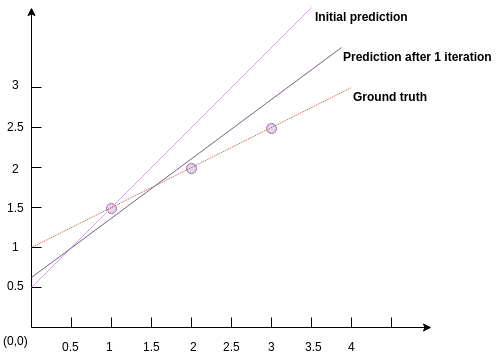
\includegraphics[scale=0.7]{background/figures/regression.png}
\caption{Example of linear regression. Here the red line is the best approximation of a y value, given an x value.} 
\label{fig:regression_example}
\end{figure} 
Figure \ref{fig:regression_example} shows an ideal example of linear regression with the model we are solving. Here we approximate the values of our model with the straight line defined by choosing the right slope (a) and the right constant (b).
With the knowledge of math, we look into how to do it computationally with the help of machine learning. 


We can recall from the quote \ref{ML} by \cite{MitchellTomM1997Ml} that we gain experience E by doing a task T. In our example we choose to store our experience as its done in equation \ref{eq:ML_lin}.
    
\begin{equation}
y=W^{(0)}x+W^{(1)}\\
\label{eq:ML_lin}
\end{equation}

\noindent Here, like before, our output is y, and our input is x. We have replaced ``a'' and ``b'' with new placeholders $W^{(0)}$ and $W^{(1)}$. In this example  $W^{(0)}$ and $W^{(1)}$ are constants, but in more complex examples, $W$ would be matrices.
Now our goal is to, given a task T, gain experience E and store it in $W^{(0)}$ and $W^{(1)}$. With our values for $W^{(0)}$ and $W^{(1)}$ we want the best performance P.  The best performance here is defined as getting the smallest difference between the predicted output data and the actual output data. 

\noindent The most prominent way of calculating this error is to use the mean square error between the predicted and actual output of the data. 
\begin{equation}\label{eq:MSE_form}
     MSE=\frac{1}{2m} \sum_i (\hat{y}-y)_i^2 =\mathcal{L}
\end{equation}

Where $m$ is the number of samples, $y$ is the real output, and $\hat{y}$ is the predicted output. The 2 in the denominator is just a constant to make the derivation of the formula easier.\\
From this, we can intuitively see that the error tends towards 0 when $\hat{y}$=$y$. We can also note, because of the squaring in the formula, that the error is only based on L2\footnote{The L2 distance is the Euclidean distance between two points in a plane. L1 distance, often called Taxicab distance, taking the absolute value instead of the square root.} distance between $\hat{y}$ and $y$.\\
Now that we have an error, we need a way to improve it.
At this point, we have a way to store experience E (in  $W^{(0)}$ and $W^{(1)}$), measure performance P (in the MSE), and we have tasks T (in the form of input-output pairs).
Given an input-output pair, we will now look at how to use machine learning to better approximate the next input-output pair.

\vspace{5px}
Lets start with: 
\begin{equation}
    x=\left[ \begin{array}{c} 1\\ 2\\ 3\\ \end{array} \right],
    y=\left[\begin{array}{c} 1.5\\2\\ 2.5\\\end{array}\right]
\label{eq:input}
\end{equation}
As we can discern from this formula, and by looking at the Figure \ref{fig:regression_example}, our ideal model would lie at $y=0.5x + 1$ as marked with the dotted red line. This means that our ideal weights would be  $W^{(0)}=0.5$ and $W^{(1)}=1$.
In our initial formula, we set the the weights $W^{(0)}=1$ and $W^{(1)}=0.5$. To get the ideal formula, we would like $W^{(0)}$ decrease by a half and $W^{(1)}$ to increase by a half.
Using the formula \ref{eq:ML_lin} with the input $x$ values we can calculate $\hat{y}$, given our weights, to be:
\begin{equation}
    \hat{y}=\left[\begin{array}{c} 1.5\\ 2.5\\ 3.5\\ \end{array}\right]
\end{equation}
We can now calculate the performance by applying an error function. Using the MSE formula \ref{eq:MSE_form}, the loss $\mathcal{L}$ is:
\begin{equation}
   \mathcal{L} = \frac{1}{2*3} \left( {(1.5-1.5)}^2+{(2.5-2)}^2+{(3.5-2.5)}^2 \right) = 0.20
\end{equation}
With our new found error, we need a way to use this to update our weights $W^{(0)}$ and $W^{(1)}$ to get a better estimate. 
    

\noindent The most common way to update our weights is to use gradient descent. 
Gradient descent is a first order iterative optimisation algorithm for finding the minimum of a function~\cite{robbins1951}. In our case, we are looking for the minimum value of the MSE function. Gradient descent is defined as (simplified for our example):
\begin{equation}
    a_{n+1}= a_{n} - \gamma \nabla F(a_{n})
    \label{eq:gradientdecent}
\end{equation}
Where $\nabla$F is the derivative of the function in question, a is the input at step n, and $\gamma$ is a learning rate set to a small number. The learning rate is an essential part of the calculation, as without it we would often calculate the new weights too extreme for our problem. By introducing a learning rate, we take small, more controlled steps in the right direction. 

\noindent Derivating \ref{eq:MSE_form} and using a learning rate of 0.2 we get the following. 
\begin{equation}
    \label{MSE_deriv_w0}
    \begin{split}
    \nabla F_{W^{(0)}} &= \frac{d}{d_{W^{(0)}} } \frac{1}{2m} \sum_i (\hat{y}-y)_i^2 \\
     &= \frac{1}{m} \sum_{i}{(\hat{y}-y)}_{i} \cdot x_i\\
     &= \frac{1}{m} \sum_{i}{(W^{(0)} \cdot x + W^{(1)}-y)}_{i} \cdot x_i\\
    \end{split}
\end{equation}

\begin{equation}
    \label{MSE_deriv_w1}
    \begin{split}
     \nabla F_{W^{(1)}} &= \frac{d}{d_{W^{(1)}} } \frac{1}{2m} \sum_i (\hat{y}-y)_i^2 \\
                    &= \frac{1}{m} \sum_{i}{(\hat{y}-y)}_{i} \\
                    &= \frac{1}{m} \sum_{i}{(W^{(0)} \cdot x + W^{(1)}-y)}_{i}\\
    \end{split}
\end{equation}
\noindent Inserting \ref{MSE_deriv_w0} and \ref{MSE_deriv_w1} in to \ref{eq:gradientdecent} gives us the two following formulas for $W^{(0)}$ and $W^{(1)}$
\begin{equation}
    \label{GD_W0}
    \begin{split}
    W^{(0)}  &= W^{(0)} - \gamma \frac{1}{m} \sum_{i}{(W^{(0)} \cdot x_i + W^{(1)}-y)}_{i} \cdot x_i \\
              &= 1 - 0.2 \cdot \frac{1}{3}  \sum (0+1+3)  \\
              &= 0.733\\
    \end{split}
\end{equation}
\begin{equation}
    \label{GD_W0}
    \begin{split}
    W^{(1)}  &= W^{(1)} - \gamma \frac{1}{m} \sum_{i}{(W^{(0)} \cdot x_i + W^{(1)}-y)}_{i} \\
              &= 0.5 - 0.2 \cdot \frac{1}{3} \sum (0-0.5-1) \\
              &= 0.6\\
    \end{split}
\end{equation}

\noindent The new weights gives us $\hat{y}$ to be:
\begin{equation}
    \hat{y}=\left[\begin{array}{c} 1.25\\ 1.85\\ 2.45\\ \end{array}\right]
\end{equation}
This gives us the loss:
\begin{equation}
   \mathcal{L} = \frac{1}{2*3} \left( {(1.33-1.5)}^2+{(2.06-2)}^2+{(2.79-2.5)}^2 \right) = 0.019
\end{equation}

\noindent After one iteration of gradient descent, we see the weights becoming closer to the desired result. With more iterations the closer the weights will get to the point that gives the smallest error, as long as the learning rate is small enough. 
We looked at an example using the formula for a linear approximation. In the real world, there are only a handful of problems that we \textbf{can} solve by making a linear approximation. We will now look into more advanced types of approximations made with machine learning.

    

\section{Neural Networks}
We have looked at different types of machine learning, and we have gone in depth into how a linear regression model works. In this section, we want to get further insight into how we can make more complex models, and we will look into the most popular method for machine learning, namely neural networks~\cite{haykin1994neural}. 
After the rundown on how neural networks are built up and how they operate, we will look into convolutional neural networks. In the end, we will look at successful networks, mainly made for image generation and classification which is our target challenge in the medical domain. 


\subsection{The perceptron}
\label{cha:perceptron}
To explain how a neural net operates, we first need to look at the most fundamental structure present in every type of neural network, namely the perceptron.
Frank Rosenblatt introduced the first perceptron in 1957 as an attempt to mimic the human neuron~\cite{perceptron}.  


\begin{figure}[h]
        \centering
        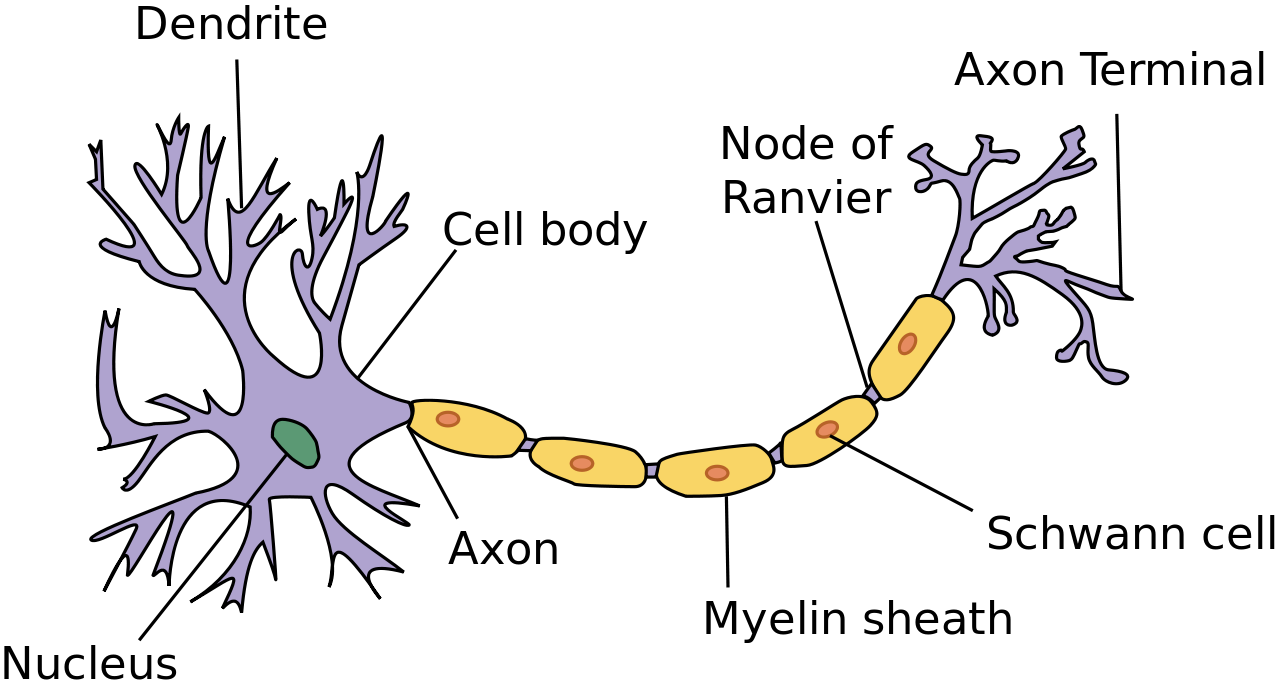
\includegraphics[scale=0.3]{background/figures/neuron.png}
        \caption{Image of a simplified neuron}
        \label{fig:neuron}
\end{figure}


Figure \ref{fig:neuron}\footnote{From \url{https://commons.wikimedia.org/wiki/File:Neuron.svg}} shows what a human neuron look like, and in which direction the signal goes. Each neuron is connected to multiple other neurons by connecting the dendrites to other neighbouring neurons forming a pathway for the electrical signals to flow. 
When a signal is sent, the dendrites register the signal and sends it through the axon out to the axon terminal. At the axon terminal, other neurons pick up the electrical signal and pass it through their axon.
This flow of electricity is the fundamental way different part of our brain communicates, and the different pathways the signals can take represent how we learn. The original idea behind the perceptron and this branch of machine learning is to mimic this process of making pathways throughout the network as a way to learn from experience.


\begin{figure}
        \centering
        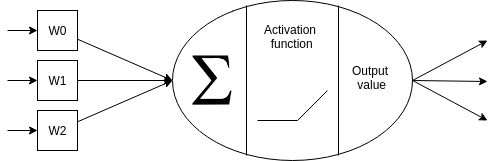
\includegraphics[scale=0.7]{background/figures/perceptron.png}
        \caption{Simple perceptron that sends out an output that is the tanh of the the sum of the inputs}
    \label{fig:perceptron}
\end{figure}




With the biological neuron as a reference point, we can now look more in-depth into the mathematical equivalent. 
Figure \ref{fig:perceptron} shows the equivalent in the realm of computer science, having the same flow from the input to the output. 
The perceptron does, however, not work with electrical signals. Instead, it works with numbers representing this signal. This abstraction gives the perceptron the ability to have arbitrary high values, as well as negative ones. 
We multiply the input signals to the perceptron with an associated weight. In biological terms, this weight is equivalent to the strength of the connection between the two neurons trying to communicate. We sum together the weighted inputs and apply a threshold function. In the first perceptron, the internal function were:


\begin{equation}
    \label{eq:tresh}
 f_{out}=   \left\{
\begin{array}{ll}
		1 \ \ if \ \ \textbf{W} \cdot \textbf{x} + b > 0, \\
     	0 \ \ otherwise \\
\end{array} 
\right. 
\end{equation}
where $\textbf{x}$ is the input, $\textbf{W}$ is a vector of real-valued weights, $\textbf{w} \cdot \textbf{x}$ is the dot product $\sum _{i=1}^{m}w_{i}x_{i}$, where m is the number of inputs to the perceptron, and b a constant bias. 


The general formula of the perceptron is unchanged, though we have moved away from the ``0-1 output'' perceptron in favour for more complex output functions like the sigmoid in 1989~\cite{Funahashi:1989:ARC:71287.71290}, the ReLu and tanh in the 2000s. 

\begin{equation}
    \label{eq:ReLu}
 f_{out}=   max\left\{
\begin{array}{ll}
		\textbf{w} \cdot \textbf{x} + b \\
     	0 \\
\end{array} 
\right. 
\end{equation}
The typical ReLu preceptron.



\subsection{Feed Forward and Backpropagation Through the Perceptron}
The general concept of the learning process is similar to the one we presented in section \ref{cha:concept}. To better understand the function of a perceptron we will explain the same steps as we saw in the linear regression example, only for our perceptron.

First our perceptron gets signals $x_{(i,0)}-x_{(i,n)}$ where $n$ is the number of inputs to the perceptron (for instance three in Figure \ref{fig:perceptron}). The signals received is the input in the same way as we received an input an array in equation \ref{eq:input}.
For each of the input values, $x_{(i,0)}-x_{(i,n)}$, we multiply it by a weight $W^{(0,0)}$ -  $W^{(0,n)}$. Here, in contrast to the linear regression example, every input has its own weight.
After the weight multiplication, we sum the result to a scalar.
We are now almost ready to give the result as an output, but to prevent the perceptron of only being able to solve linear problems when connection multiple perceptrons, we need to use an activation function. This activation function can be ReLu as in equation \ref{eq:ReLu}, or something like tanh or Sigmoid shown in Figure \ref{fig:activations}. Note that we do not use the threshold function in equation \ref{eq:tresh} as an activation function in modern neural networks, as it is not applicable for gradient descent.

Now that we have an output, we look at the error between the output $f_{(j,0)}$ and the expected output and apply a loss function. We can now backpropagate the error to update the weights at the start of the perceptron.


\subsection{Multilayer perceptrons}
\label{cha:MLP}
The neural network was a proposal made by Warren McCulloch and Walter Pitts (1943)~\cite{roweis2000nonlinear}. They created a computational model for neural networks based on mathematics and algorithms called threshold logic. 

The first multilayer network at the time used backpropagation with gradient decent in the same way described in equation \ref{eq:gradientdecent}.

\begin{figure}[h]
\centering
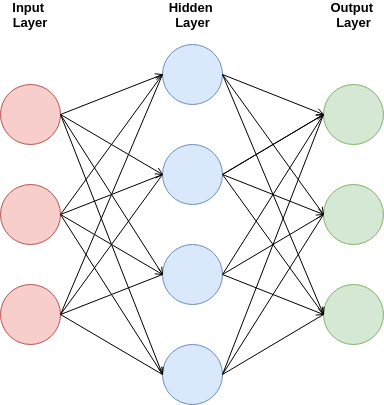
\includegraphics[scale=0.7]{background/figures/neural_network.png}
\caption{Simple illustration of a multilayer perceptron with three inputs, one hidden layer with four nodes, and one output layer with three nodes.}
\label{fig:mlnn}
\end{figure}


Figure \ref{fig:mlnn} shows the basic structure of a multilayer network. This model has one hidden layer and the standard input and output layers. In our figure, each of the nodes is a perceptron\footnote{In reality the input layer does not usually behave as a perceptron with an activation function. The input layer is only there to propagate the signal to the neurons further into the network.} as described in section \ref{cha:perceptron}, and each vertex is the weight between the corresponding perceptrons. For a model like the one in Figure \ref{fig:mlnn}, we need 20 placeholders to store our weights. The number of weights also increases with the number of perceptrons equal to the number of perceptrons in each layer multiplied together. 

The advantage of using the multilayer structure proposed by McCulloch and Pitts is the fact that we are not constricted to a linear boundary classification model. By using the multilayer structure the network can, for instance, tackle the XOR problem, not solvable by a single layer neural network. 




    
\subsection{Convolutional Neural Networks}
\label{cha:convNet}
The multilayer perceptron we have discussed is a robust tool that can learn a multitude of decision boundaries, and subsequently learn to classify thousands of different classes. 
As we get more data and more classes, the networks needed to solve our problem also need to grow. We can recall from section \ref{cha:MLP} that the number of weights between neurons is $i \cdot j$ where i is the first layer and j is the connected second layer. As the number of perceptrons per layer in our neural networks increases, the total amount of storage space increases too. 

Given that we want to classify colour images to recognise if an image is of a dog or a cat, we first want to feed the whole image with all three colour channels into our network.
\begin{equation}
    \label{eq:weights_l}
     height_i \cdot width_i \cdot \ channels_i \cdot height_j \cdot width_j \cdot \ channels_j  = weights
\end{equation}
Given an image with height and width of 128 pixels connected to the same shape in a network with a fully connected layers, the total amount of weighs per connection  are:\\
\begin{equation}
    \label{eq:weights_n}
     (128\cdot 128\cdot 3) \cdot (128\cdot 128\cdot 3) = 2415919104  = 2.4\cdot 10^9
\end{equation}

Given that we are working with quadratic images, the number of weights increases with a factor of four as we increase the layer height and width. As we saw in equation \ref{eq:weights_n}, the number of parameters for a relatively small image is already $2.4 \cdot 10^9$, not including the bias on top.
The models we use to store our data saves the weighs as float32, which means that each weight is 4 bytes of storage. That means that the total storage for this \textit{single} layer is:
\begin{equation}
    \label{eq:weights_GB}
    4\text{b} \cdot 2.4 \cdot 10^9 = 9,66 \ \ \text{GB}
\end{equation}
Given that a standard computer usually have 8-16 GB of RAM, this one layer might not be able to load at all. 
 



Another problem with the standard MLP is the fact that it is spatially dependent. Given an input $x$, the output, $y$, of the MLP will vary a lot if we shift the input data by one place, or if we flip the data. In some cases, this is something we want in our machine learning algorithms, but more often this behaviour is not a desirable outcome.
Given the downsides we have with regards to memory usage and non-spatiality in our multilayer perceptrons, we present Kunihiko Fukushima~\cite{Fukushima1980} solution to solve both complications.
Convolutional neural networks (CNN) are the most popular form for image recognition, segmentation, and classification~\cite{NIPS2012_4824}~\cite{Long_2015_CVPR}.
When building a convolutional neural network we often use multiple layers stacked on top of each other to give the network traits that a regular multilayer perceptron could not achieve. By far the most essential layer of the convolutional neural network is the convolutional layer.


\subsubsection{Convolutional layers}

Convolutional networks work with filters as opposed to perceptrons with weights assigned before and after the input in the vertices between perceptron as shown in Figure \ref{fig:conv_opp}. Convolutional layers assign a weight to each position in a special filter matrix. This use of filters significantly reduces the number of weights between layers, since we now have weights that are not dependent on the input size, and only dependent on this matrix size.

The three main parameters of a convolutional layer are the number of filters, kernel size and strides.
When making a convolutional layer, we start by pseudo-randomly initialising a $ (F \times K \times K)$ matrix as our weights.
In this matrix, F is the number of filters in the convolutional layer and K is the filter size. We can think of this as F filters of size $(K \times K)$ stacked on top of each other. 
When applying the convolutional layer to an input vector, we take each of the F filters and slide it over the image. 
For each position of the filter, we multiply the image value with the filter and sum the result. The scalar made by this multiplication is the value passed on to the next layer at that specific point.
Figure \ref{fig:conv_opp} shows this convolution process after 3 sliding operations with a $(3 \times 3)$ filter. When sliding across the image we have the option to take larger strides for the sliding window, in practice this striding still ``see'' the entire image, but the number of output connections are $\frac{1}{stride}$.
 
\begin{figure}[h]
        \centering
        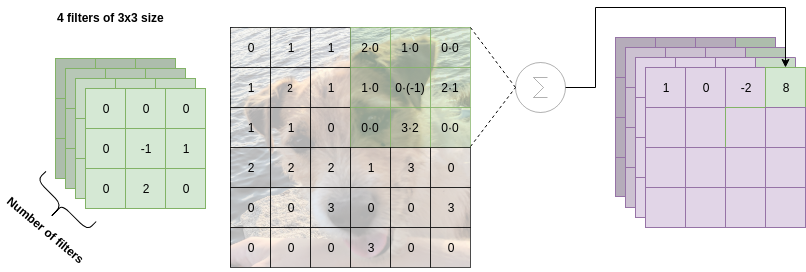
\includegraphics[scale=0.5]{background/figures/Conv_filter.png}
        \caption{The values calculated when a convolutional filter after 4 sliding window operations, here the number of inputs does not represent how many inputs there usually is in an image}
        \label{fig:conv_opp}
\end{figure}


As we can see from this architecture, we only change the weights in the filter matrix, as there are no other variables in the convolutional operation. Using this sliding window technique gives us the benefit that the filter only gathers information from the local area, and subsequently makes the convolutional operation non-spatially dependent.  

\subsubsection{Activation layers}
As we discussed in section \ref{cha:perceptron}, in addition to summing the inputs and passing them on, we need to apply an activation function to the output. The encounter same problem with our desire to make non-linear problems, apply in the CNN model. 
To apply an activation layer to a CNN, we take every value in the matrix and apply the activation function separately to every data-point. 

In this thesis, our CNNs used only the three activation functions shown in Figure \ref{fig:activations}, with slight modifications.
\begin{figure}[h]
        \centering
        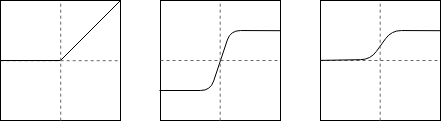
\includegraphics[scale=0.8]{background/figures/activations.png}
        \caption{Activation functions from -2 to 2 on each axis. \\ From left to right: ReLu, Tanh, Sigmoid}
        \label{fig:activations}
\end{figure}

\subsubsection{Pooling}
\label{cha:pool}
Pooling layers, often also called downsampling layers, are commonly found in CNN's. 
Their primary role in the network is to reduce the spatial size of the data provided, and thus reducing the number of weights and variables used by the network. This reduction helps with reducing processing and memory costs.  
The two most common pooling operations are max pooling and average pooling~\cite{zhou1988computation}\todo{MICHAEL OR PAAL:\\ I have not read this because its behind a paywall.. This is the same reference that was used in \url{https://www.deeplearningbook.org/contents/convnets.html} by Ian Goodfellow, so I believe its legit}. Both methods resemble convolutions in the way that they apply their function to a sliding filter over the data. 
 
\begin{figure}
        \centering
        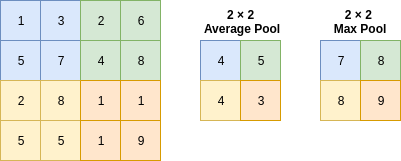
\includegraphics[scale=0.7]{background/figures/pooling.png}
        \caption{Both max and average pooling done on a 4 $\times$ 4 matrix}
        \label{fig:pooling}
\end{figure}

Just like in Figure \ref{fig:pooling} the most common pooling parameters are of filter size 2 and stride 2. Using this configuration leaves every point of the input checked once, and the resulting output size is halved. 
Pooling layers do generally not have any weights associated with them. This lack of weights means that the pooling layer routes the signal back without changing it during backpropagation.

In addition to the pooling described above, we in this thesis use global pooing in addition to regular pooling. Global Max pooling and Global average pooling works with individual layers of the convolutional net, taking the max or average of the whole feature map instead of using a sliding filter, as shown in Figure \ref{fig:GAP}.
Global pooling has the effect of transforming the network from 3 dimensions to 1 dimension, making this layer ideal right before any fully connected layers at the end of longer networks.

\begin{figure}
        \centering
        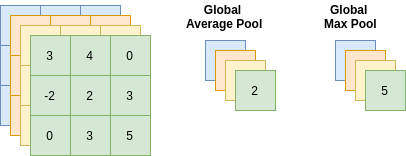
\includegraphics[scale=0.7]{background/figures/GAP.png}
        \caption{Global pooling. Here, each of the four layers gets averaged or maxed in to a scalar, giving us a 1D vector at output}
        \label{fig:GAP}
\end{figure}

\subsubsection{Normalisation}
\label{cha:normalisation}
Training deep neural networks can often be complicated with the fact that the distribution of each layer changes during training, as the parameters of the previous layers change. In some cases, this constant shift of input values slows down the training by requiring a lower learning rate to keep the network stable.
We refer to this problem as internal covariate shift, and we use normalisation as a tool to correct for it~\cite{DBLP:journals/corr/IoffeS15}.

The most common way to normalise the data is to use batch normalisation. When calculating the batch normalisation, we take the following steps presented in S. Ioffe and C. Szegedy publication: ``Batch Normalization: Accelerating Deep Network Training by Reducing Internal Covariate Shift''~\cite{DBLP:journals/corr/IoffeS15}.\\

\begin{minipage}{\textwidth}	
\noindent \textbf{Input:} Values of x over a mini-batch: $\mathcal{B} = \{x1...m\}$;\\
\noindent Parameters to be learned: $\gamma, \beta$\\
\noindent \textbf{Output:} $\{y_i = \text{BN}_{\gamma,\beta}(x_i)\}$\\
\begin{align*}
\mu_{\beta} &\leftarrow \frac{1}{m} \sum_{i=1}^{m} x_i   \tag{mini-batch mean}\\
\sigma_{\beta}^2 &\leftarrow \frac{1}{m} \sum_{i=1}^{m} (x_i-\mu_{\beta})^2 \tag{mini-batch variance}\\
\widehat{x_i} &\leftarrow \frac{x_i - \mu_{\beta}}{\sqrt{\sigma_{\beta}^2+\epsilon}} \tag{normalise}\\
y_i &\leftarrow \gamma\widehat{x_i}  + \beta \equiv \text{BN}_{\gamma,\beta}(x_i) \tag{scale and shift}
\end{align*}
\label{eq:BN}
\end{minipage}

In the original paper we the writers saw a significant reduction in the number of epochs needed to train the network, as well as increased accuracy.


\subsubsection{Dropout}
A major problem in machine learning is the act of overfitting the data. We say that a model is overfitting to the data when it learns the bias that comes with the dataset as shown in Figure~\ref{fig:dropout}. A practical way to see if a model is starting to overfit is to look at the training error versus the test error. If the training error keeps decreasing while the test error increases, we tend to believe that the model is learning the training data distribution and not generalising to unseen data.


\begin{figure}[t]
        \centering
        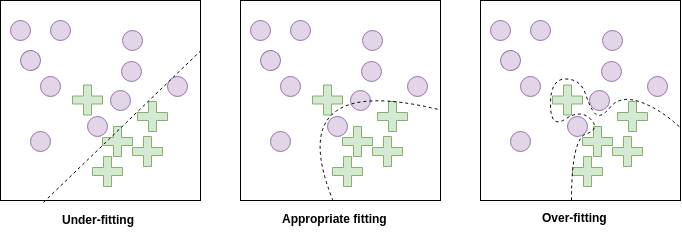
\includegraphics[scale=0.6]{background/figures/Under_vs_overfitting.png}
        \caption{Three cases of data boundary prediction. In most cases we desire appropriate amount of fitting to our dataset to keep generalisation}
        \label{fig:dropout}
\end{figure}


Dropout, first proposed by Srivastava et al.~\cite{JMLR:v15:srivastava14a}, in 2014 was used to prevent overfitting of neural networks (As seen in figure \ref{fig:dropout}).
Dropout layers in the CNN will randomly cut a certain number of connections in a layer. The number of cut connections is usually between 25\% and 50\% of the total. The result of the use of dropout is that the network can not rely on only a few numbers of weights during training since there is a chance the input from the weight will be cut at random intervals. 

This random cutting forces the network to spread out the essential weights throughout the network. 
Even though dropout does not explicitly change the weights, it implicitly forces the stong weights to be evenly distributed throughout the network. 

Another popular way to combat overfitting is to add a weight regulariser like L1 or L2 distance penalty. This penalty gives the network weights an additional penalty based on their size.
As we recall, big weights in the networks have the most significant influence on the result, as each weight is multiplied by the input. If the network finds some bias hidden in the dataset, it is much harder for it to exploit this discovery.
This difficulty is because, with L1 or L2 regularisation, the network is also penalised for strong weights.
Dropout does, in practice, the same as an L1 or L2 regulariser. 


\section{Complex Neural Network models}
We have now looked at the basic concept of the neural network, and a more in-depth look into the convolutional neural network and the relevant layers.
Our primary focus has been from a computer vision perspective, where we have looked at image classification. 
To get a better insight into the act of inpainting, we need to present two other types of network, namely the Autoencoder (AE)~\cite{Rumelhart:1986:LIR:104279.104293} and the generative adversarial network (GAN)~\cite{Goodfellow:2014:GAN:2969033.2969125}.

We often base both models on the convolutional architecture, to have the option to work with image and video data. 
Both networks are a type of unsupervised learning, where the goal is to either recreate or construct data based on the training data.

We will also present the concept of transfer learning as a tool for easier classification.


\subsection{Autoencoders}
\label{cha:Explaining_autoencoders}
An autoencoder is a neural network that is trained to recreate a copy of the input given. 
As with the networks explained at this point, it has an input, some number of hidden layers and an output. The network can be considered to have two internal structures, the encoder (denoted as $h=f(x)$) and decoder (denoted as $r=g(h)$) shown in figure \ref{fig:simpleAE}.
The general goal of the autoencoder is to recreate the input $g(f(x)) = x$, but in the real world, we often add restrictions to make the autoencoder unable to copy the input perfectly. Because of this restriction, the autoencoder is forced to prioritise particular properties of the data, and hence it might learn underlying features that define the dataset.

\begin{figure}[t]
    \centering
    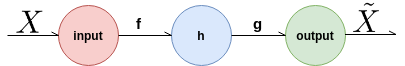
\includegraphics[scale=0.8]{background/figures/SimpleAE.png}
    \caption{The general structure of an autoencoder, encoding $\textbf{x}$ with $\textbf{f}$, then decoding $\textbf{h}$ with $\textbf{g}$ to an output $\textbf{x}$.}
    \label{fig:simpleAE}
\end{figure}

Traditionally, autoencoders were used for tasks like feature learning and dimensionality reduction, though with the rise in computing power, autoencoders are now in use at the forefront of generative modelling.

To use an autoencoder for generative modelling, we need to set an objective for autoencoder to achieve.
When generating new images we can propose regulisers to the latent space\footnote{We often call the area between the encoder and the decoder the latent space. Here the information is at its maximum compression.} between the encoder and the decoder. The reguliser might be that the output of the latent space layer should follow a Gaussian noise pattern or another easily replicable pattern. 
This type of autoencoder is called a variational autoencoder. Variational autoencoders have the advantage of being able to create new completely unseen data if Gaussian noise is inputted at the latent space, effectively cutting out the encoder and supplying random noise instead.
Another way to use an autoencoder for generative modelling is by masking areas in the input data the model used to train on, and give the unmasked data as the target output.
Figure \ref{fig:AEinpainting} shows this concept of an inpainting autoencoder. The act of inpainting forces the autoencoder to learn the underlying features of the inpainted area to make a prediction. 

\begin{figure}[t]
    \centering
    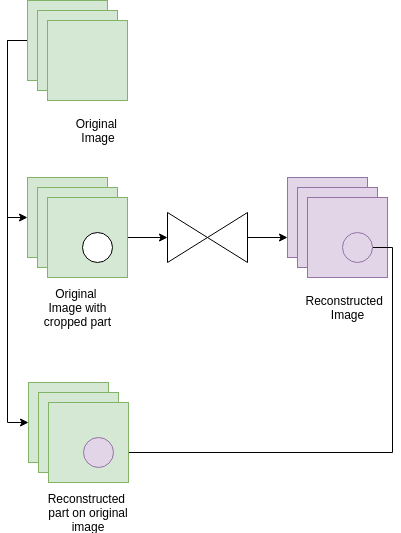
\includegraphics[scale=0.6]{background/figures/AE_for_inpainting.png}
    \caption{Autoencoder where the goal is to inpaint the masked area shown in the original dataset as a purple circle, and as a red circle generated by the autoencoder.}
    \label{fig:AEinpainting}
\end{figure}


As with supervised classifiers, autoencoders use gradient descent to optimise the result, as the model work to recreate the input $\textbf{x}$ from out output $\widetilde{\textbf{x}}$. \\    
We achieve this by minimising the loss function:\\
\begin{equation}
    \mathcal{L}(\textbf{x},g(f(\textbf{x})))
    \label{eq:AEloss}
\end{equation}
As this is a problem where the goal is to minimise error, autoencoders often use MSE or mean absolute error (MAE) as the optimiser for the gradient descent. 
As we noted earlier, Figure \ref{fig:AEinpainting} show a visual example of equation \ref{eq:AEloss} when inpainting.

\todo{Here we add an example of new AE paper perhaps}
    
\subsection{Advaserial neural networks}
\label{cha:Explaining_GANS}
As an alternative to using autoencoders for generative modelling, we introduce the generative adversarial network proposed by Goodfellow et al.~\cite{Goodfellow:2014:GAN:2969033.2969125}.

As shown in Figure \ref{fig:GAN}, the GAN consist of two components: a generative model G that captures the data distribution, and a discriminator model D that estimates the probability that the sample from G is fake, and does not come from the training data. The training procedure for the generator is to maximise the probability of the discriminator to make mistakes.
The generator-discriminator network resembles a two-player game where both parties want to ``win'' over the other.
As we are using multilayer perceptrons in our network, we can use backpropagation to train both the generator and discriminator. 

In mathematical terms:
The generator produces samples $x=g(z;\theta^{(g)})$, where $g$ is the network given the weights $\theta$. Then the discriminator network predicts if a sample is drawn from the dataset or the generator.
More specific, it gives a probably given by $d(x;\theta^{(d)})$ , and determines if $x$ is from the generator or the data-set. 
Since we have two networks competing against each other we can look at this as a zero-sum game where the generators payoff is determined by $v(\theta^{(g)},\theta^{(d)})$, and the discriminators payoff is determined by $-v(\theta^{(g)},\theta^{(d)})$.

Where $v$ is a function that is determined by both the success rate of the discriminator and the generator, the most commonly used is:
\begin{equation} 
    v(\theta^{(g)},\theta^{(d)}) \; = \; \mathds{E}_{x\sim p_{data}}\log{d(x)} + \mathds{E}_{x\sim p_{model}}\log{(1 - d(x))} 
\end{equation}
as derived from~\cite{Goodfellow:2014:GAN:2969033.2969125}.


\begin{figure}[ht!]
    \centering
    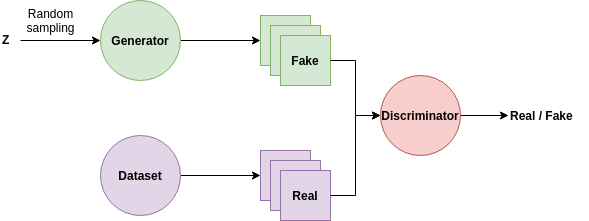
\includegraphics[scale=0.6]{background/figures/GAN.png}
    \caption{The basic concept of the generative adversarial network}
    \label{fig:GAN}
\end{figure}


\todo{Here we add an example of new gan paper, like \cite{DBLP:journals/corr/abs-1812-04948}}

    
\subsection{Transfer learning}
Neural networks are prone to overfitting when training on a small dataset or over multiple iterations. We often have problems with the fact that we need to train a network for a long time for it to learn the features associated with the data, though we often learn the bias in the dataset either in addition or instead of the features that define the dataset.

The most obvious solution is to gather more training data to prevent this overfitting, or to use regulisers to force the network to diversify the layer weights, as proposed in section \ref{cha:normalisation}.

In this thesis, we have chosen to use transfer learning to address this problem. Transfer learning is the process of using knowledge from similar problems to help solve the current goal.  Let us say we want to classify different wolf breeds without the necessary amount of data. We can use our knowledge about dog breeds to help the classification, by using a pretrained model as a base for training. Since both wolf and dogs share many of the same features, like four legs and fur, the model does not need to learn those features from scratch.
Similarly, we can use general models to help solve our specific problem.



     
   
\section{Summary}
We started the background chapter by looking at the medical procedure associated with a colonoscopy, and we went in-depth into how the medical staff work with digital equipment. We got some insight into the time and complexity invested in finding polyps when doing the said colonoscopy.
We then looked at systems for computer-aided diagnosis and the prevalent systems that is in use today to help medical staff with polyp detection. 
From this assessment, we saw that the polyp detection rate was relatively high, but polyps were often overlooked, and model-overfitting was often the cause of the high-grade results. Though the advances in medical image diagnosis, the ability for models to generalise to other areas has not come far enough.
We then took a close look at machine learning, from the building blocks in the perceptron to the complex pretrained neural networks used today in modern algorithms. 

As we noted in chapter \ref{cha:CAD}, in modern medical diagnosis systems we lack the ability to adapt to new datasets from a different distribution than the training set. We have a strong belief that this is related to the fact that we overfit the data on the training set and the fact that we learn dataset-specific features not present in other unknown datasets.


Hicks et al. in the paper \textit{``Dissecting Deep Neural Networks for Better Medical Image Classification and Classification Understanding''} goes in-depth into the problem of overfitting with regards to the problem with dataset specific features. We can see from this paper that by removing dataset specific artefacts, the classification score increased when evaluating the model on previously unseen data.

Pogorelov et al. in the paper \textit{``Deep Learning and Hand-crafted Feature Based Approaches for Polyp Detection in Medical Videos''} shows similar results when training on the small datasets and evaluating the data on different larger publicly available datasets.

In this thesis, we want to continue to explore this problem of lack of generalisation and find ways to improve models in that manner.








































































































































































































\iffalse
\subsubsection{Explain how the ML-methods can be used with the polyps}
When you work with machine learning a lot of the job is to make the data as clear as possible. \\
Imagine that you want to do something as simple as reading an analogue clock. The ``straight forward'' way to do it is to make a convolutional neural network to look at the dials. This will require a much more complex network compared to if you could convert the angle of the dials to degrees and have that as an input to your model.

    \begin{figure}[ht]
      \centering
      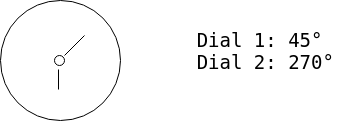
\includegraphics[scale=0.5]{methods/figures/Clock.png}
      \caption{A clock needs a more complex network compared to just the degrees}
    \end{figure}
    %TODO FIND ORIGinal source
    The trick is often to make the data as refined as possible. 
    Further, some of the techniques used are described.
    



\section{In painting}
  We have discussed the importance of good input data, and the potential benefits to resource usage and ease of making a good model.
  So a priority when it comes to image classification is to have data without anomalies and other areas that can be interpreted as a feature for the classifier. 
  In a machine learning perspective, the data is best if it has the same structure, and is %TODO similar enough.
  In painting is the process of reconstructing lost or deteriorated parts of images and videos. %TODO CITE https://en.wikipedia.org/wiki/Inpainting
  

  From previous papers on polyp detection in the GI tract %TODO CITE!!!
We have clear results that the black corners and the green squares trigger a big activation %TODO WRITE BETTER
  when it comes to classifying images. 
  From %TODO CITE, find out who
  's paper, we can see that the activation map on a regular image gives a very high result on, in addition to the polyp, the corners and the green square. 
  \begin{figure}[ht]
    \centering
    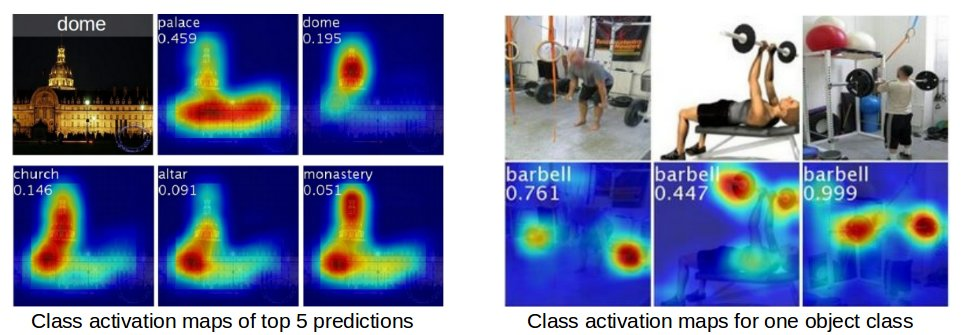
\includegraphics[scale=0.5]{background/figures/placeholder.jpeg}
    \caption{Using X's activation map we can see that the edges triggers unwanted activations}
  \end{figure}
  
  In addition to squares and edges, we also have the problem that parts of the image is over saturated at points where the light from the led is reflected directly back to the camera.
  Another problem is when the camera captures images that are too close to the wall. Both of these scenarios creates patches where the saturation is maximum. 
   \begin{figure}[ht]
    \centering
    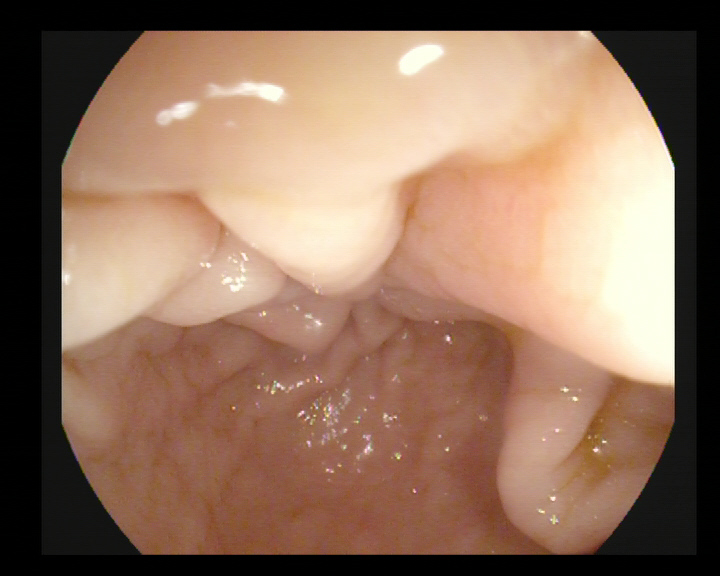
\includegraphics[scale=0.5]{background/figures/reflection.jpg}
    \caption{we have two different types of saturation: the reflected area in the top part of the image, and the right side of the image.}
  \end{figure}
  in an ideal scenario, the image would have no pixel values at max, and as little frame as possible. 
  We, therefore, want to make a tool that can help us with this.
  \subsection{Naive methods for In painting}
    Inpainting is not a new area of research, as it has been around since %TODO CITE
    Because of this, there are many naive methods that give good inpaintings. 
    
    \subsubsection{Textured syntesys based on image inpainting}
    \subsubsection{MOARE}
    \subsubsection{MOARE}
   \subsection{Naive methods for borderfinding}

%
% THIS SECTION MUST BE MOVED/FIXED
%
\section{Naive Methods REM}
      Now that we have an idea of what we are looking for we can first turn to some more naive methods for detecting anomalies, and for enhancing the images.\\
      The field of image processing has been researched since\\ %TODO WHEN
      
      Using some of the classic methods in image processing, we can see if\\ %TODO
      
      We often describe the method into two groups of information: First and Second order statistics.\\
      \textbf{First order:} First order statistics does not take in to account the relative positioning of the pixels in the image, and because of this, gives much less information than the second order statistics.\\
      Example of First-order statistics is often what information we can get out of a histogram. This can be skewness, variance, and mean value.\\
      
      \vspace{10px}
      
      \textbf{Second order:} Second-order statistics takes in to account the relative positioning of the pixels in the image. We can calculate the GLCM matrix and get a much more detailed view of the image. \\
      
      
      
      \subsection{GLCM}
        A GLCM (Grey-level co-occurrence matrix) is a matrix that is used when examining the spatial relationship of pixels in a texture. 
        The calculation of a GLCM gives us how often pairs of pixels with specific values and a specified spatial relationship occur at a given place in an image. %TODO CITE
      
        \subsubsection{Algorithm}
          For simplicity we use only greyscale in this example:
          \begin{figure}[ht]
        \centering
        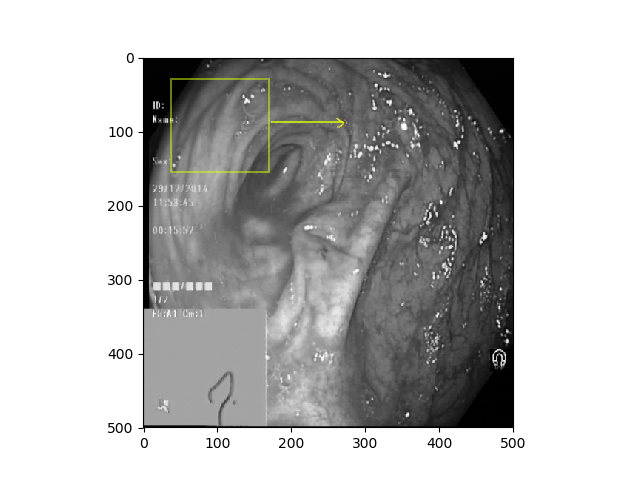
\includegraphics[scale=0.5]{figures/sliding_window_box.png}
        \caption{GLCM capturing features}
          \end{figure}
          The algorithm starts by running a sliding window over the image, often with a stride, and for each stop calculates the spatial relationship between each pixel specified.
          The result can be something like this figure %TODO link to figure
          where we can read out the most likely neighbouring pixel.
           \begin{figure}[ht]
        \centering
        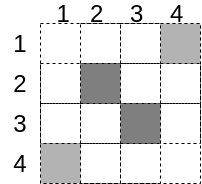
\includegraphics[scale=0.5]{figures/Simple_GLCM.png}
        \caption{GLCM Matrix}
          \end{figure}
          The darker colours on in the matrix are indicating that we often have a jump between, for instance, pixel-value of 1 and a pixel value of 4, but no from 1 to 1.\\
          With this information, we can get a naive pattern-recogniser. 
        \subsubsection{Other uses}
          Besides for the pattern recognition we can use the GLCM to get the information on:
          \begin{itemize}
           \item \textbf{Contrast} is the difference in luminance or colour in the picture. We would expect low contrast in the “background” and higher contrast around edges and irregular objects.
           \item \textbf{Homogeneity} is how similar a local area is to itself
           \item \textbf{Variance} $\sigma^2$ , is directly a measure of ”roughness”
           \item \textbf{Mean} value of a GLCM can give us areas with higer or lower pixel values. Good way to find polyps if they are lighter than the tissue around.
           \item \textbf{Entropy}
           \item \textbf{Energy}
          \end{itemize}


      
      \subsection{Edge detection}
        Using Edge detection in is another viable way to look for polyps. 
        \begin{figure}[ht]
          \centering
          \begin{minipage}[b]{0.45\textwidth}
        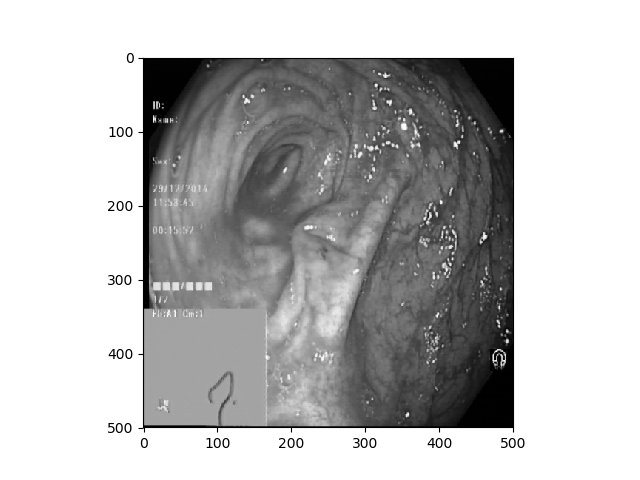
\includegraphics[width=\textwidth]{figures/sliding_window.png}
        \caption{Original image}
          \end{minipage}
          \hfill
          \begin{minipage}[b]{0.45\textwidth}
        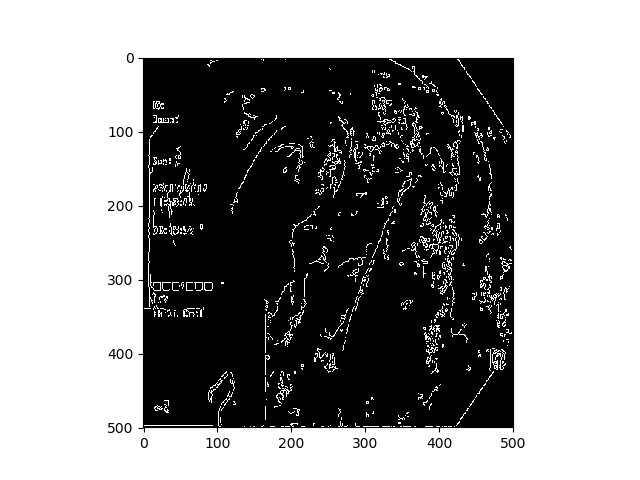
\includegraphics[width=\textwidth]{figures/Canny.png}
        \caption{Edges of the picture}
          \end{minipage}
        \end{figure}
        \subsubsection{Algorithm}
          For each pixel look at the neighbouring pixel, if \\
          
          \begin{centering} 
        $ abs(p_a - p_b)>tresh $\\ 
          \end{centering}
          
          then mark a pixel as an edge pixel. \\
          
      \subsection{Hough Transforms}
        Using, for instance, Canny edge detection %TODO CITE
        we can get a better view of where the potential border of the polyp/anomaly is. (As shown in %TODO FIG CITE)
        
        A Hough transform can I theory have many/any shape(s), and together with edge detection, we might find some of the polyps this way.
        
    
    
    
    
    
    
    As we can see from this, there are a lot of old methods that can give approximations. We can also conclude that none of these methods is perfect.
    We will, therefore, look at methods that take learning in to use.
\section{Using machine learning for inpainting}
    \subsection{AE}
    \subsection{CE}
    \subsection{CCGAN}
    \subsection{PCNN}
    As discussed earlier, machine learning is using prior experiences to make decisions given the problem at hand. 
    It is also worth mentioning that we do not need labelled data since we are in a way looking at a global average of every image both with and without polyps. We are therefore incentivised to use an 
    Unsupervised approach.
    Since machine learning is learning from a training set, it is essential that the training set contains as little as possible of the features we want to remove. \\
    
    Because of this, the first thing we need to do if we are going to mask out corners and squares is to limit the training set only to contain cropped, non-square images. 
 
    \begin{figure}[ht]
      \centering
      \begin{minipage}[b]{0.45\textwidth}
    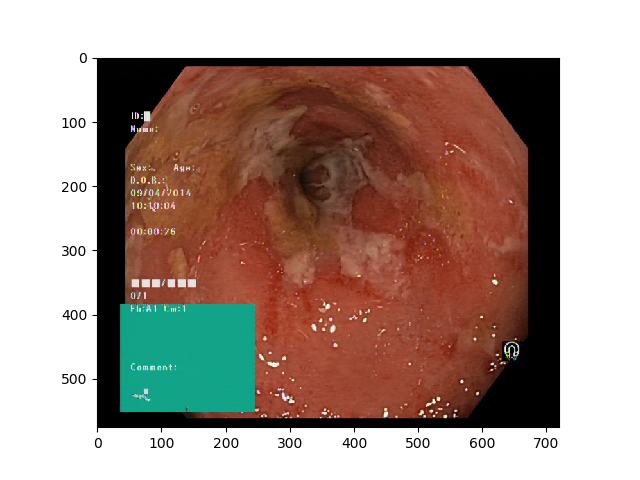
\includegraphics[width=\textwidth]{background/figures/uncropped_img.png}
    \caption{Original image with black padding}
      \end{minipage}
      \hfill
      \begin{minipage}[b]{0.45\textwidth}
    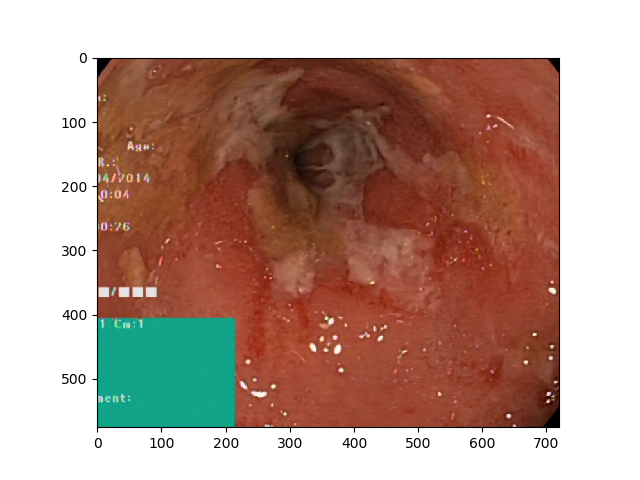
\includegraphics[width=\textwidth]{background/figures/cropped_8percent_img.png}
    \caption{Black edges cropped away + 8\% zoom}
      \end{minipage}
      \caption{Here we have an example on how we would make an image better to train on. This is not representative of the training since we only use images without the green square under training}
    \end{figure}
    
    Now that we have better images to train our data with, we need the correct algorithm.
    We have already seen unsupervised learning aproaches in chapter %TODO ref 
    \newpage
    \subsubsection{Algorithm}
      \todo{Hvordan skal jeg gaa frem nar det kommer til aa presantere disse? skal jeg bare si hvilke metoder jeg har testet?}
      Text about presenting UML, and stuff.
  
    \newpage
    As we recall from earlier, an autoencoder is a type of neural network that tries to output a recreation of the output.\\%TODO: REF the part about autoencoders 
    We can use this for inpainting by setting the algorithm to train on images with areas cropped away.
    There are a couple of different ways we can train an autoencoder to do this.\\
    
    %\todo{shouldI talk about the different ways or present the best?}
    
    
    \vspace{10px}
    \textbf{Denoising Autoencoder with MSE loss:}\label{par:Denoising_Autoencoder_with_MSE_loss}\\
    The simplest way to train the autoencoder is to first take the trainingset $\mathds{X}$ and make an augmented copy $\widetilde{\textbf{x}}^{(i)}$ for 
    every data point in $\textbf{x}_{\sim \mathds{X}}^{(i)}$. \\
    \textit{Here $\widetilde{\textbf{x}}$ is a copy of x with random areas masked.}\\
    
    Now we minimise the loss function\\    
      \begin{equation}
        L(\textbf{x},g(f(\widetilde{\textbf{x}})))
      \end{equation}
    over the whole image.\\
    \vspace{20px}
    
    With this approach, the autoencoder learns to fill in the blank spots with credible data, without changing the rest of the image. 
    \todo{this will probably work best if the autoencoder is not under complete, perhaps talk about this}
    One problem by this approach is that we do not want the rest of the image to change for obvious reasons, and the algorithm as it is here has the flaw that it will change all the pixels in the image, at least to a minor degree. \\
    
    This can be somewhat fixed by only taking the augmented parts, and pasting them directly into the image. This will leave most of the original image, except for the parts that were cropped randomly.\\
    
    \vspace{10px}
    \textbf{Denoising Autoencoder with \todo{clever tittle}:}\\
    If we take what we learned from \ref{par:Denoising_Autoencoder_with_MSE_loss}, we can make a more optimal autoencoder:
    Rather than taking a loss like     
    \begin{equation}
      L(\textbf{x},g(f(\widetilde{\textbf{x}})))
    \end{equation}
    over the whole image, we can rather just focus on the parts that matters, namely the cropped areas.\\
    
    If we add the cropped image to the output from the autoencoder to make an image, we can use this new image to train out loss.
    For most of the image, the loss will be zero, since the only part that is changed is the cropped area. 
    We can also make a new loss that is more optimal for the task at hand. 
    \begin{equation}
      MSE_{crop}\:=\: \frac{1}{n}
      \begin{cases}
          \begin{array}{lcl}
          (\widetilde{\textbf{x}}-\textbf{x}) \; if \; \widetilde{\textbf{x}} \: \in \: \textbf{x}_{crop} \\
          0 \; else
          \end{array}
      \end{cases}
    \end{equation}
    Where $\textbf{x}_{crop}$ is the area that was cropped away from the original image and $n$ is the number of pixels in that area.\\
    With this modified MSE we are assured that only the pixels in the cropped area is changed with gradient decent, and we save a lot of computation as an added bonus.
    
    
    \todo{token to not train}
    \begin{figure}[ht!]
        \centering
        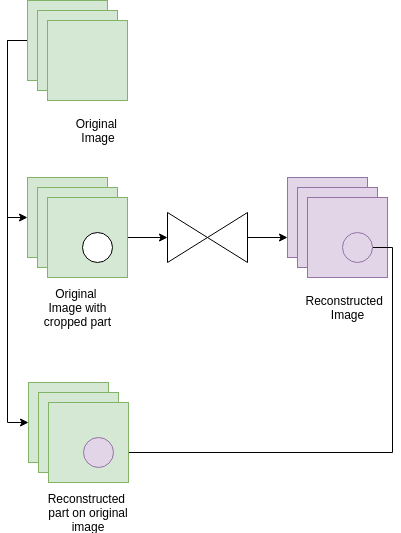
\includegraphics[scale=0.5]{background/figures/AE_for_inpainting.png}
        \caption{Final result of the autoencoder used in the testing}
    \end{figure}
    
    
    
    
    
      \subsubsection{Explaining GANs, this will be moved}
      
    
      \subsubsection{Contextencoder}
    Inpainting can also be done with adversarial models, and using a network trained to do the task of inpainting can be a lot more powerful than using just an autoencoder\todo{ref} or the naive methods\todo{ref}.
    A contextencoder is building on the adversarial principle by using a generator/discriminator pair to fill in masked areas in an image. 
    
    The concept behind a Contextencoder is to take the whole image as input to an encoder/decoder pair and \todo{finish}
    
    
    
      \subsubsection{CCgan}
      \subsubsection{PixelCNN}
      
\fi

  
 
